\newpage

\section[Программная реализация]{\large \centering Программная реализация}
\hspace{\parindent} Разработанный алгоритм реализован на языке программирования C++ без использования сторонних библиотек и может быть запущен на всех основных операционных системах: Windows, Linux, Mac OS. Кроме основного приложения, был создан веб-интерфейс, через который также можно получить выравнивание. Так как задача требует существенных вычислительных ресурсов, практично запускать программу на мощной вычислительной платформе, а осуществлять взаимодействие с ней через веб-интерфейс. Кроме этого, для возможности внедрения отдельных компонент программы в другие проекты, были собраны статические библиотеки построения парного и множественного выравниваний.

\subsection[Структуры данных]{\large Структуры данных}
\hspace{\parindent} Ниже описанны используемые в программе структуры для хранения и обработки кодирующих последовательностей. Всего разработано и реализовано три объекта: структура $BioSeq$, описывающая биологические последовательности, класс построения парного выравнивания $PairwiseAlign$ и структура $Profile$ для работы с набором последовательностей. Все они входят в состав собранных статических библиотек и могут быть легко подключенны в другие проекты.

\subsubsection[Представление биологических последовательностей]{\large Представление биологических последовательностей}
\hspace{\parindent} Для представления биологических последовательностей используется структура $BioSeq$ (листинг~\ref{lst:BioSeq}) с двумя строковыми полями:
\begin{itemize}
	\item $name$ --- идентификатор последовательности
	\item $nt\_seq$ --- последовательность нуклеотидов
\end{itemize}

Ради удобства использования у нее определен оператор индексирования [ ] и функция $Length$, возвращающая текущую длину последовательности. Чтобы иметь связь нуклеотидного и аминокислотного уровней, реализованы методы, позволяющие получить как трансляцию всей строки по первой рамке считывания $std::string$ $GetAAseq()$ $const$, так и конкретного триплета, начинающегося с $i$-го индекса $char$ $TranslateNTtoAA(int$ $i)$ $const$. Также необходимо иметь возможность вставлять разрывы в последовательность, для чего были добавлены методы $InsertGap(int$ $pos)$ и $InsertGap(int$ $pos,$ $int$ $count)$, добавляющие $1$ или $count$ разрывов по индексу $pos$. Печать реализована через перегруженную операцию $<<$. В качестве результат работы программы желательно получить выравнивание не только на нуклеотидном, но также и на аминокислотном уровне. Для наглядного разделения этих двух опций, в структуру были добавлены методы $void$ $PrintNT(std::ostream\&$ $out)$ и $void$ $PrintAA(std::ostream\&$ $out)$, которые выводят результат выравнивания и его трансляцию соответственно в указанный поток $out$.
\begin{algorithm}
	\caption{Структура представления биологических последовательностей BioSeq} \label{lst:BioSeq}
	\begin{lstlisting}
struct BioSeq {
  std::string name;
  std::string nt_seq;
  // constructor
  BioSeq(std::string n, std::string s): name(n), nt_seq(s) { }
  // destructor
  ~BioSeq() { }
  // accessors
  int Length() { return nt_seq.length(); }
  char operator [] (int index) { return nt_seq[index]; }
  void InsertGap(int pos, int count);
  void InsertGap(int pos);
  // translater
  std::string GetAAseq() const;
  char TranslateNTtoAA(int i) const;
  // printer
  void PrintAA(std::ostream& out);
  void PrintNT(std::ostream& out);
  friend std::ostream& operator << (std::ostream& stream,
                                    const BioSeq& data);
};
	\end{lstlisting}
\end{algorithm}

\subsubsection[Класс построения парного выравнивания]{\large Класс построения парного выравнивания}
\hspace{\parindent} Вычисление оптимального выравнивания двух последовательностей реализовано через  класс $PairwiseAlign$ (листинг~\ref{lst:PairwiseAligner}). Таким образом, в одном объекте собираются и данные, и методы их обработки, что упрощает импорт алгоритма парного выравнивания в другой проект.\\
\indent Класс не содержит полей с исходными последовательностями, в нем хранятся только структуры для построения ответа и параметры выравнивания: штрафы за разрывы, смещение рамки, появление преждевременного стоп-кодона, матрицы замен нуклеотидов и аминокислот. Данные для выравнивания передаются через метод $Align(const$ $BioSeq*$ $seq1,$ $const$ $BioSeq*$ $seq2)$, реализующий алгоритм из пункта~\ref{PairwiseAlign}. Однако, для увеличения производительности вместо рекурсии происходит заполнение таблицы оптимальных ходов, как в классическом алгоритме Нидлмана-Вунша.\\
\indent Для хранения матриц замен используются два массива: $nt\_score\_matrix$ (нуклеотиды) и $aa\_score\_matrix$ (аминокислоты), размерностью $128\cdot 128$ элементов, так как символы строк представлены одним байтом, принимающим значения от 0 до 127 (рисунок~\ref{ris:memory}).
\begin{figure}[H]
	\center{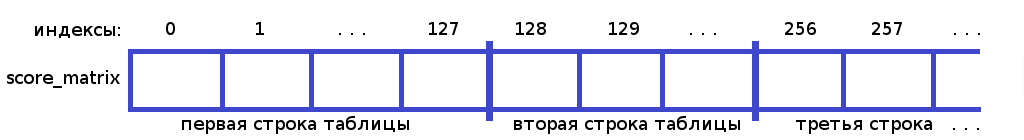
\includegraphics[width=0.75\linewidth]{memory.png}}
	\caption{Представление матрицы замен в памяти компьютера}
	\label{ris:memory}
\end{figure}
\indent Используя данный подход, на вход программе выравнивания можно подавать последовательности с символами из произвольного алфавита, необходимо лишь определить соответствующие матрицы замен и предоставить функцию для перевода кодонов. Адресация определена следующим образом:
\begin{equation*}
nt\_score\_matrix[(unsigned\hspace{0.2cm} char)'A'*128+(unsigned\hspace{0.2cm} char)'C']
\end{equation*}
Полученное значение --- цена за сопоставление аденина ($A$) и цитозина ($C$). В общем случае, вместо конкретных нуклеотидов, в формулу подставляются $i$-ый и $j$-ый символы строк: $seq1[i]$, $seq2[j]$.

\begin{algorithm}
	\caption{Класс построения оптимального выравнивания двух последовательностей} \label{lst:PairwiseAligner}
	\begin{lstlisting}
class PairwiseAlign {
private:
  int gap_open, gap_extension, gap_frame, stop_cost;
  int nt_score_matrix[128*128];
  int aa_score_matrix[128*128];
  int seq1_length, seq2_length; 
  int matrix_size = 0;
  int* F = NULL; // score matrix
  int* W = NULL; // way matrix
  void NewScoreMatrix(const char* file_name, int* score_matrix);
  
public:
  PairwiseAlign(const char* nt_score_matrix, 
      const char* aa_score_matrix, int stop_cost, int gap_open, 
      int gap_extension, int frame_gap);
  ~PairwiseAlign() { if (F) delete[] F; if (W) delete[] W; }
  
  // calc align 
  int Align(const BioSeq* seq1, const BioSeq* seq2);
  std::pair<std::string, std::string> GetAlign();
  
  // change substitution matrices
  void ChangeNTscoreMatrix(const char* file_name) {
    return NewScoreMatrix(file_name, nt_score_matrix);
  }
  void ChangeAAscoreMatrix(const char* file_name) {
    return NewScoreMatrix(file_name, aa_score_matrix);
  }
  
  // accessors
  int GetGapOpen() { return gap_open; } 
  int GetGapExtension() { return gap_extension; } 
  int GetGapFrame() { return gap_frame; } 
  int GetStopCost() { return stop_cost; } 
};
	\end{lstlisting}
\end{algorithm}

\subsubsection[Профили]{\large Профили}
\hspace{\parindent} Выравненные строки сохраняются в структуру $Profile$ (листинг~\ref{lst:ProfileStruct}). Для экономии памяти и времени в профили заносятся не копии последовательностей, а только указатели на них. Функция объединения записана в виде перегруженной операции $+$. Кроме этого, профили имеют методы для вычисления оценки за сопоставление двух столбцов нуклеотидов и аминокислот. Так же, как и для структуры $BioSeq$ реализована возможность вставки разрывов по указанному индексу заданной длины. Дополнительно, у профилей имеется массив $frequency$, содержащий частоты распределения нуклеотидов и аминокислот в конкретной позиции. Для его заполнения реализованы методы $CalcFrequenciesNT$ и $CalcFrequenciesAA$.\\
\begin{algorithm}
	\caption{Структура профилей} \label{lst:ProfileStruct}
	\begin{lstlisting}
struct Profile {
  Profile();
  ~Profile();
  // data
  std::vector<BioSeq*> sequences;
  int frequency[128];
  // alignment of two profiles
  Profile& operator + (Profile& another);
  // alignment of profile and sequence
  Profile& operator + (BioSeq* sequence);
  // get score in column
  float ColumnNTscore(BioSeq* seq, int index1, int index2);
  float ColumnAAscore(BioSeq* seq, int index1, int index2);
  float ColumnNTscore(Profile& another, int index1, int index2);
  float ColumnAAscore(Profile& another, int index1, int index2);
  // fill an array of frequency
  void CalcFrequenciesNT(int position);
  void CalcFrequenciesAA(int position);
  // insert gaps in sequences
  void InsertGap(int pos, int count);
  void InsertGap(int pos) {
    for_each(sequences.begin(), sequences.end(), 
      [pos] (BioSeq* s) {
        s->nt_seq.insert(pos, 1, '-');
      }
    );
  }
};
	\end{lstlisting}
\end{algorithm}


\indent При работе с профилями необходимо гарантировать, что ни одна из входящих в его состав последовательностей не будет модифицирована или удалена до конца построения выравнивания. В противном случае возможно появление ошибок выполнения или ухудшение качества результата. 

\subsection[Общая схема работы]{\large Общая схема работы}
\hspace{\parindent} На рисунке~\ref{ris:scheme} показана общая блок-схема работы программы. Основные этапы реализованы в виде отдельных, независимых друг от друга блоков, которые впоследствии можно модифицировать или заменить новыми. 
\begin{figure}[H]
	\center{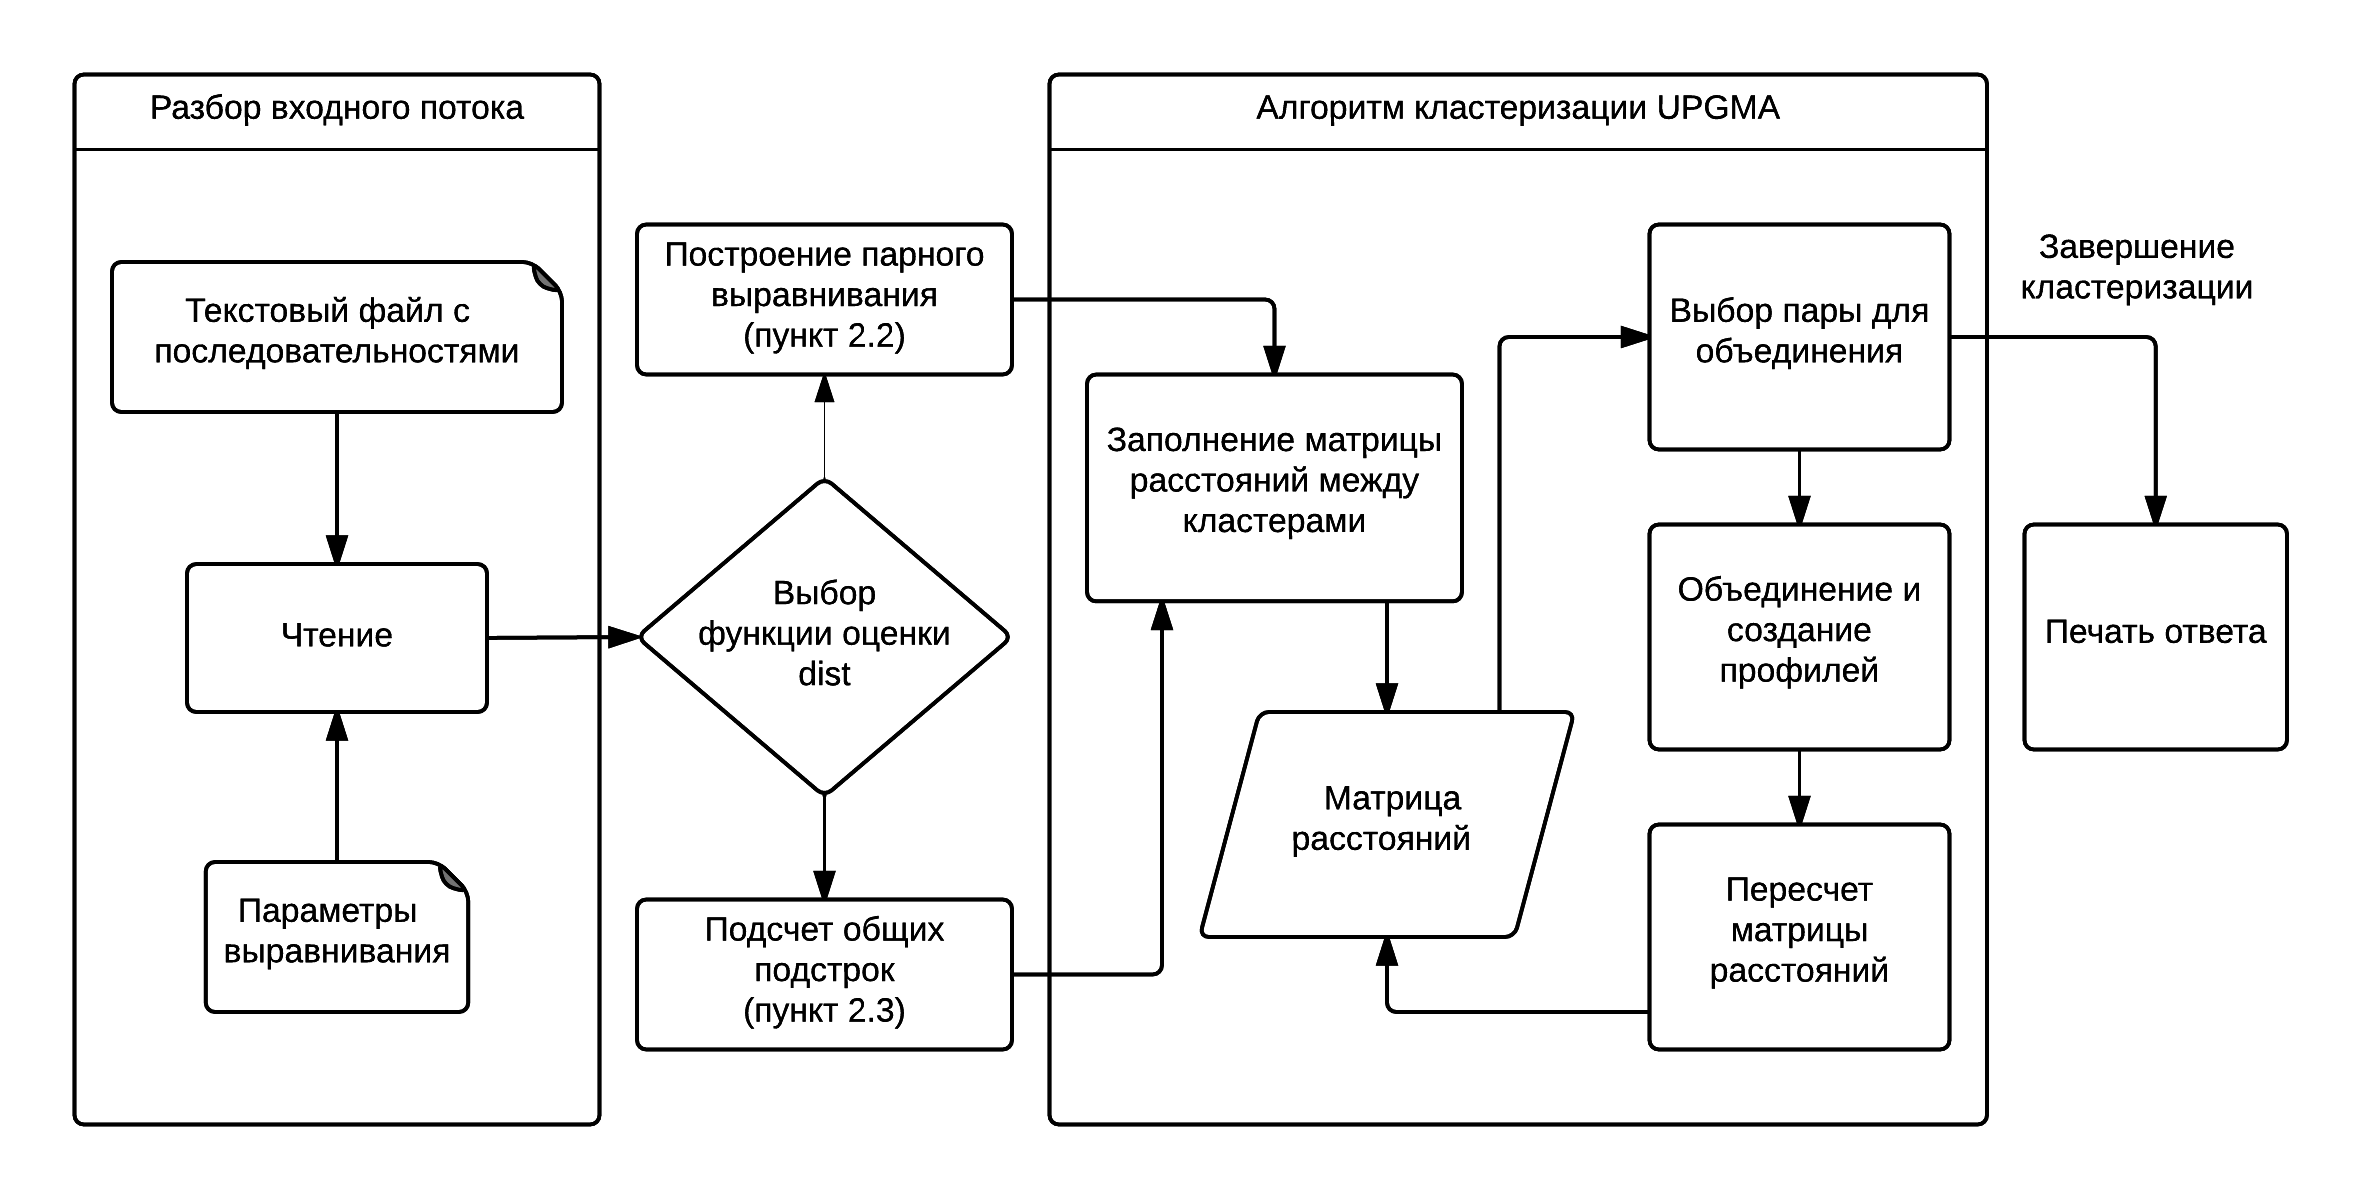
\includegraphics[width=1.\linewidth]{block-scheme.png}}
	\caption{Блок-схема работы программы}
	\label{ris:scheme}
\end{figure}

\subsubsection[Чтение входных данных]{\large Чтение входных данных}
\hspace{\parindent} На вход программе подается текстовый файл с последовательностями в формате FASTA~\cite{FASTAformat}. Строка, начинающаяся с символа '>', называется строкой описания. Она содержит имя последовательности и некоторую дополнительную информацию, предназначенную для идентификации. Другие строки, начинающиеся с символа ';', являются комментариями и игнорируются. За строкой описания следует код последовательности. При кодировании нуклеотидов буквами A, C, G и T кодируют, соответственно, аденин, цитозин, гуанин и тимин. На рисунке~\ref{ris:FASTAexample} представлен пример тестового файла в формате FASTA.
\begin{figure}[H]
	\center{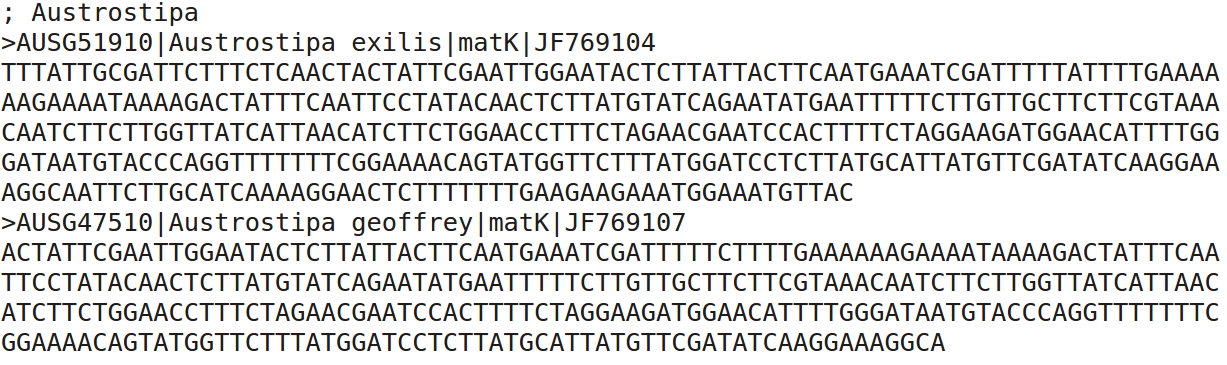
\includegraphics[width=1.\linewidth]{FASTAexample.png}}
	\caption{Пример файла в формате FASTA}
	\label{ris:FASTAexample}
\end{figure}

Программа может использовать для вычисления очков за сопоставление нуклеотидов и аминокислот пользовательские матрицы замен. Их необходимо представить в таком же формате, как и на рисунке~\ref{ris:BLOSUM62}.
Строки, начинающиеся с символа $\#$, являются комментариями и игнорируются, а при задании таблицы первые строка и столбец определяют символы сопоставления. Количество пробелов может быть любым.

\begin{figure}[h]
	\center{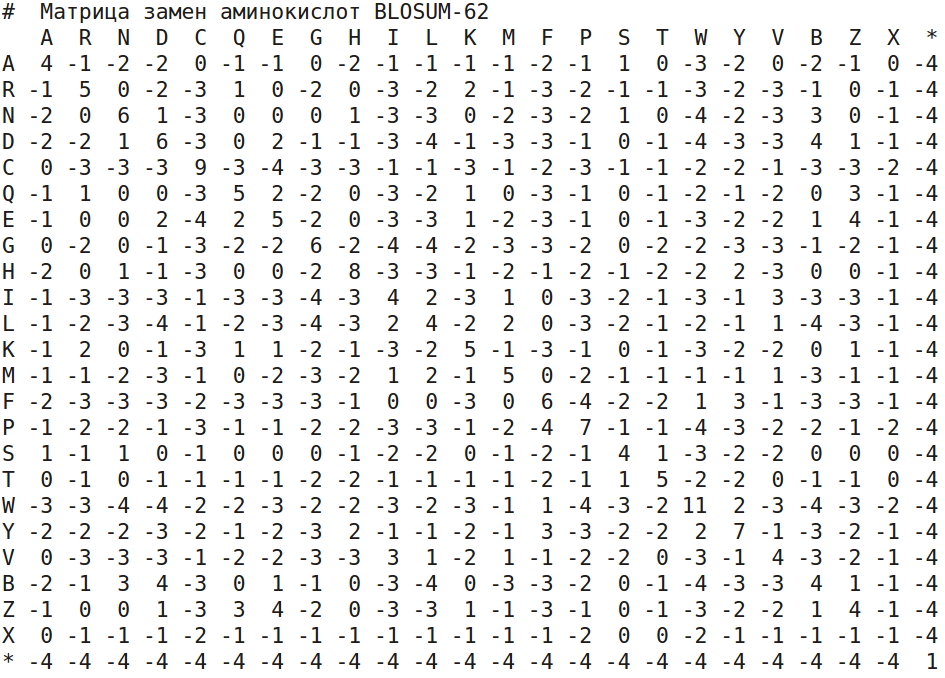
\includegraphics[width=0.9\linewidth]{BLOSUM62.png}}
	\caption{Пример файла с матрицей замен}
	\label{ris:BLOSUM62}
\end{figure}

\subsubsection[Определение порядка выравниваний]{\large Определение порядка выравниваний}
\hspace{\parindent} Алгоритм кластеризации реализован в виде процедуры, принимающей на вход массив последовательностей и функцию оценки расстояния между ними --- $dist$. Пользователь может выбрать, что использовать в качестве оценки $dist$: метод построения парного выравнивания $Align$ из класса $PairwiseAlign$ или подсчет количества одинаковых подпоследовательностей заданной длины $k$. Для использования своей собственной функции расстояния ее необходимо определить как $std::function<int$~$(BioSeq*$, $BioSeq*)>$. \\
\indent На каждом шаге алгоритма не происходит выделение новой памяти для перехода от старой таблицы размерности $n$ к новой $n-1$. Используется дополнительный массив, в котором хранится информация о том, какие строки и столбцы матрицы более не активны и пропускаются при переборе. 

\subsubsection[Объединение профилей]{\large Объединение профилей}
\hspace{\parindent} При объединении профилей $P_1$ и $P_2$ происходит рассчет оптимального выравнивания с заполнением матрицы размерности $len(P_1) \cdot len(P_2)$. Для того чтобы сократить количество выделений памяти, было решено сохранять заполненную таблицу после операции объединения. Таким образом, новая память будет выделена только в том случае, если текущая размерность матрицы, оставшейся с предыдущей итерации, не удовлетворяет размерности очередной пары профилей.

\subsection[Руководство пользователя]{\large Руководство пользователя}
\hspace{\parindent} Работа с программой представлена в двух вариантах: через консольное приложение или веб-интерфейс. В таблице~\ref{tabular:options} перечислены все возможные опции для запуска.
\begin{table}[H]
\caption{Опции программы}
\label{tabular:options}
\begin{center}
\begin{tabular}{|p{2.4cm}|p{3.5cm}|p{5.2cm}|p{4.4cm}|}
\hline
Короткие опции& Длинные опции& Значение& Комментарий\\
\hline
$-h$& $--help$& без аргумента& вывод справочной информации\\
\hline
$-i$& $--input$& путь к файл с последовательностями & FASTA формат\\
\hline
$-n$& $--NT\_subst$& путь к файлу с матрицей замен для нуклеотидов & по умолчанию +4 за совпадение, -5 иначе\\
\hline
$-a$& $--AA\_subst$& путь к файлу с матрицей замен для аминокислот& значение по умолчанию BLOSUM62\\
\hline
$-g$& $--gap\_open$& штраф за открытие разрыва& значение по умолчанию -10\\
\hline
$-e$ & $--gap\_extension$& штраф за продолжение разрыва& значение по умолчанию -3\\
\hline
$-f$& $--gap\_frame$& штраф за разрыв рамки& значение по умолчанию -15\\
\hline
$-s$& $--stop\_cost$& штраф за преждевременное появление стоп-кодона& значение по умолчанию -50\\
\hline
$-d$& $--dimension$& начальная размерность матрицы для объединения профилей& значение по умолчанию 1024$\times$1024\\
\hline
$-k$& $--k-mers$& необязательный аргумент $k$& сравнение подстрок для функции $dist$; по умолчанию $k=10$ \\
\hline
$-p$& $--pairwise$& без аргумента& использование парного выравнивания для функции $dist$\\
\hline
\end{tabular}
\end{center}
\end{table}

На рисунке~\ref{ris:webka} изображен графический интерфейс для работы с программой. Форму можно условно разделить на две части: поле ввода данных и область задания параметров выравнивания. 

\begin{figure}[h]
	\center{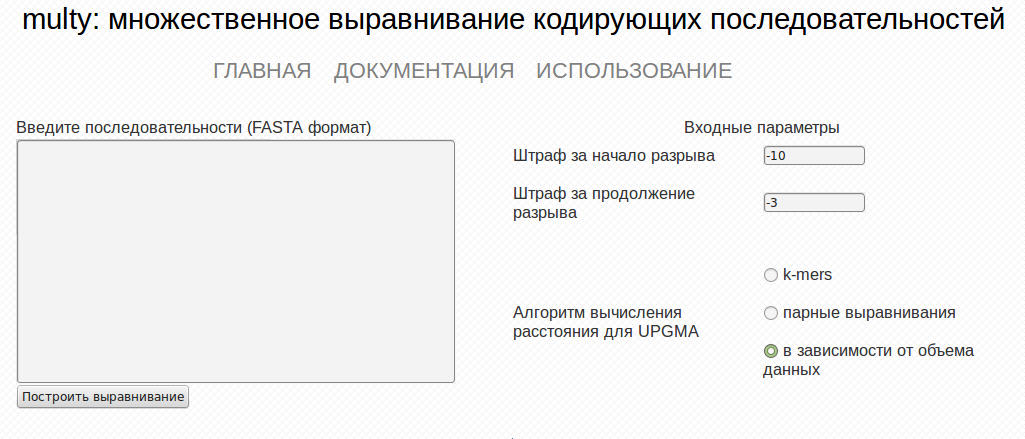
\includegraphics[width=1.0\linewidth]{web.png}}
	\caption{Графический интерфейс для построения выравнивания}
	\label{ris:webka}
\end{figure}

После ввода последовательностей и указания необходимых параметров необходимо нажать на кнопку <<построить выравнивание>>. По окончании работы будет загружена страница с результатами выравнивания (рисунок~\ref{ris:webkares}).

\begin{figure}[h]
	\center{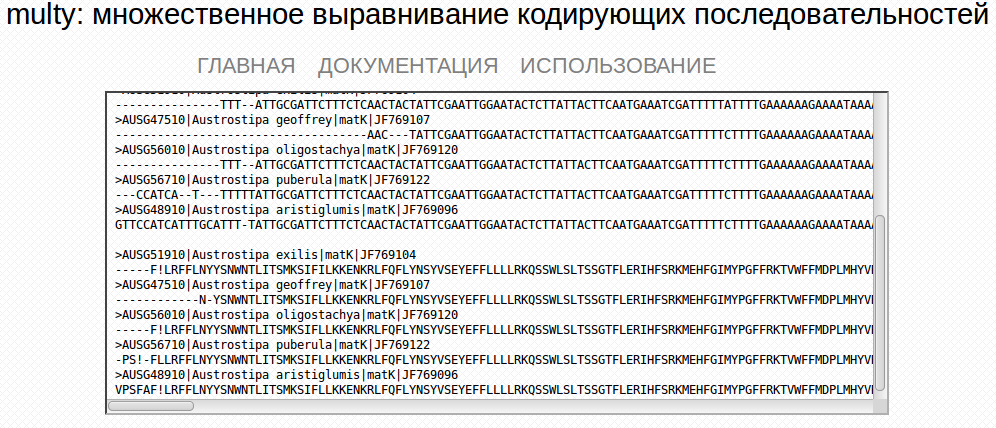
\includegraphics[width=1.0\linewidth]{webres.png}}
	\caption{Форма с результатами выравнивания}
	\label{ris:webkares}
\end{figure}